\documentclass[10pt,a4paper,twocolumn]{article}
\usepackage[T1]{fontenc}
\usepackage{mathptmx}
\usepackage[margin=0.72in,columnsep=0.25in]{geometry}
\usepackage{amsmath,amssymb}
\usepackage{graphicx,booktabs,multirow}
\usepackage[hidelinks]{hyperref}
\usepackage{algorithm,algpseudocode}
\usepackage{tikz}
\usetikzlibrary{positioning,arrows.meta,fit}
\usepackage{titlesec}
\usepackage{enumitem}
\usepackage[font=small,labelsep=period]{caption}
\usepackage{cite}

\renewcommand{\thesection}{\Roman{section}}
\renewcommand{\thesubsection}{\Alph{subsection}}
\titleformat{\section}{\centering\normalsize\scshape}{\thesection.}{0.5em}{}
\titleformat{\subsection}{\normalsize\itshape}{\thesubsection.}{0.5em}{}
\titlespacing*{\section}{0pt}{1.2ex}{0.8ex}
\titlespacing*{\subsection}{0pt}{1ex}{0.5ex}
\renewcommand{\thetable}{\Roman{table}}
\DeclareCaptionLabelFormat{tablab}{\textsc{#1 #2}}
\captionsetup[table]{labelformat=tablab,labelsep=newline,justification=centering,textfont=sc}
\captionsetup[figure]{name=Figure}
\setlength{\textfloatsep}{8pt plus 2pt}
\setlength{\floatsep}{6pt plus 2pt}

\newcommand{\passk}[1]{\mathrm{pass}^{#1}}
\newcommand{\passat}[1]{\mathrm{pass@}#1}

\title{\vspace{-1.2em}\Large Measuring the Reliability of LLM Agents: Repeated Trials, Tool Faults\\and Long Request Chains in a Simulated Customer-Service Shop}
\author{
\begin{tabular}{ccc}
Moomena Asad & Maha Asghar & Aatqa Rehman\\
\small i230054@isb.nu.edu.pk & \small i230010@isb.nu.edu.pk & \small i230012@isb.nu.edu.pk
\end{tabular}\\[2pt]
\small National University of Computer and Emerging Sciences (FAST-NUCES), Islamabad, Pakistan}
\date{\vspace{-2em}}

\begin{document}
\maketitle

\noindent\textbf{\textit{Abstract}---Agent benchmarks usually report one success rate per task, which says little about
whether an agent will do the same task correctly every time. We built a small, fully checkable customer-service
environment (five tools, four policies, 12 orders) and ran two open-weight models, gpt-oss-120b and gpt-oss-20b, with
two agent designs, ReAct and a plan-then-execute agent with a final action audit. Units were run five or ten times.
After removing infrastructure failures the analysis covers 1,760 episodes on 30 hand-solved tasks, two paraphrases per
task, injected tool faults and chains of two to four customer requests. Single-run success hides a lot. With 20\% of
tool calls failing, gpt-oss-20b still reaches pass@1 0.81, but only 40\% of the tasks succeed in all ten runs
($\passk{10}$ 0.40). Chains are worse. gpt-oss-120b solves 0.99 of single tasks but 0.13 of four-request chains
(eight chains, ten runs each), where independent per-message errors would predict 0.97. On the same four-request
chains, the plan-then-execute agent raised success from 0.05 to 0.70 (gpt-oss-120b) and from 0.00 to 0.50
(gpt-oss-20b), at about 22,000 tokens per episode, but gave no gain on three-request chains. With one run per task,
the order of the two models was reversed or tied in up to 60\% of resamples, and the ranking of all settings settled
only at nine to ten runs. Task descriptors predict which tasks will be unreliable on unseen tasks (AUC 0.88), and trace
features flag failed chain episodes after the fact (AUC 0.85). Code and logs are released with the paper.}

\smallskip
\noindent\textbf{\textit{Index Terms}---LLM agents, reliability, $\passk{k}$, fault injection, tool use, evaluation
methodology.}

\section{Introduction}
Large language model (LLM) agents now take actions in software that has consequences: they cancel orders, issue refunds
and edit records. For this kind of use the useful question is not whether an agent can do a task but whether it does it
correctly every time it is asked. Most agent benchmarks still answer the first question. SWE-bench reports one resolve
rate per model~\cite{swebench}, and the METR time-horizon metric measures the length of tasks a model completes half of
the time~\cite{metr}. A 50\% success level is a useful capability measure, but a support agent that refunds the right
amount half the time is not deployable.

Three recent lines of work point at the gap. $\tau$-bench introduced $\passk{k}$, the probability that all $k$ runs of
a task succeed, and showed it falling below 25\% at $k=8$ for GPT-4o in its retail domain~\cite{taubench}.
ReliabilityBench added paraphrased tasks and injected tool faults and found that clean-condition scores overstate
behaviour under stress~\cite{reliabilitybench}. A study of computer-use agents traced run-to-run variation to vague task
wording and changing strategies, not only to sampling noise~\cite{cua}. Surveys of agent evaluation list reliability,
long-horizon interaction and the cost of repeated trials among the open problems~\cite{kdd,yehudai,gabauer,chowa}.

We ran a small, controlled study on these questions. Our testbed is a mock online shop in which every task has a
hand-checked final database state, so success is decided exactly and never by an LLM judge. On it we compare two model
sizes and two agent designs under four conditions, with five or ten runs per unit. The paper makes five contributions:
\begin{enumerate}[leftmargin=*,itemsep=0pt,topsep=2pt]
\item A checkable testbed of 30 tasks, including 11 that must be fully or partly refused, plus frozen paraphrases, a
reproducible fault injector and a chain builder that joins tasks on different orders into one conversation.
\item A measurement of the gap between pass@1 and $\passk{k}$ up to $k=10$ under paraphrases and tool faults for
gpt-oss-120b and gpt-oss-20b~\cite{gptoss}.
\item Evidence that chain success falls much faster than an independent-errors model predicts, over chains of two, three
and four requests, and a paired comparison showing that a plan-then-execute agent with an action audit recovers much of
the loss on four-request chains, with its cost per run.
\item A run-budget analysis (E5) over one to ten runs per task that asks when model comparisons and rankings stop
changing.
\item Two predictors: a task-level classifier for which tasks will be unreliable, and an episode-level detector of
failed runs from trace features, both tested on tasks they never saw.
\end{enumerate}

\section{Related Work}
\textbf{Capability benchmarks.} SWE-bench frames 2,294 real GitHub issues as agent tasks; the best model in the original
paper, Claude 2, resolved 1.96\%~\cite{swebench}. AndroidArena tests agents on cross-app phone tasks and finds failures
in planning, exploration and reflection~\cite{androidarena}. METR's 50\% time horizon reached about 110 minutes for o3
and has doubled roughly every seven months since 2019~\cite{metr}. All three report how often a task is solved, not how
consistently.

\textbf{Reliability benchmarks.} $\tau$-bench pairs an LLM-simulated user with a tool-using agent in retail and airline
domains and judges success by the final database state~\cite{taubench}; our success check follows the same idea.
ReliabilityBench defines a reliability surface over repeated trials $k$, perturbation level $\epsilon$ and fault rate
$\lambda$, reports a drop from 96.9\% to 88.1\% under perturbation, and finds that ReAct held up better than Reflexion
under stress~\cite{reliabilitybench}. Its scale is small (1,280 episodes, two models), which is also true of ours. The
computer-use study on OSWorld uses paired McNemar and Wilcoxon tests and reports about 78\% pass@10 against about 36\%
$\passk{10}$ for a strong agent~\cite{cua}.

\textbf{Surveys.} The KDD survey organises agent evaluation by what is measured and how, and notes that reliability
guarantees and long interactions are rarely tested~\cite{kdd}. Yehudai et al.\ call for cost-efficient and fine-grained
evaluation~\cite{yehudai}. A PRISMA review of 30 publications finds no shared benchmark standards and weak
reproducibility~\cite{gabauer}, and a review of 108 papers lists reliability among the main open
challenges~\cite{chowa}.

\textbf{Agent designs.} ReAct interleaves reasoning and tool calls~\cite{react}. Reflexion adds verbal self-feedback
across attempts~\cite{reflexion}, and plan-and-solve prompting asks the model to plan before acting~\cite{planandsolve}.
Our second agent combines a plan step with a check that is computed from tool results, not from the model's own memory.

\textbf{Metrics.} We use the unbiased pass@$k$ estimator of Chen et al.~\cite{codex} and the matching unbiased
$\passk{k}$ estimator. To our knowledge none of the papers above asks how many runs per task are needed before rankings
stabilise; Section~\ref{sec:e5res} addresses this.

\section{Testbed}
\begin{figure*}[t]
\centering
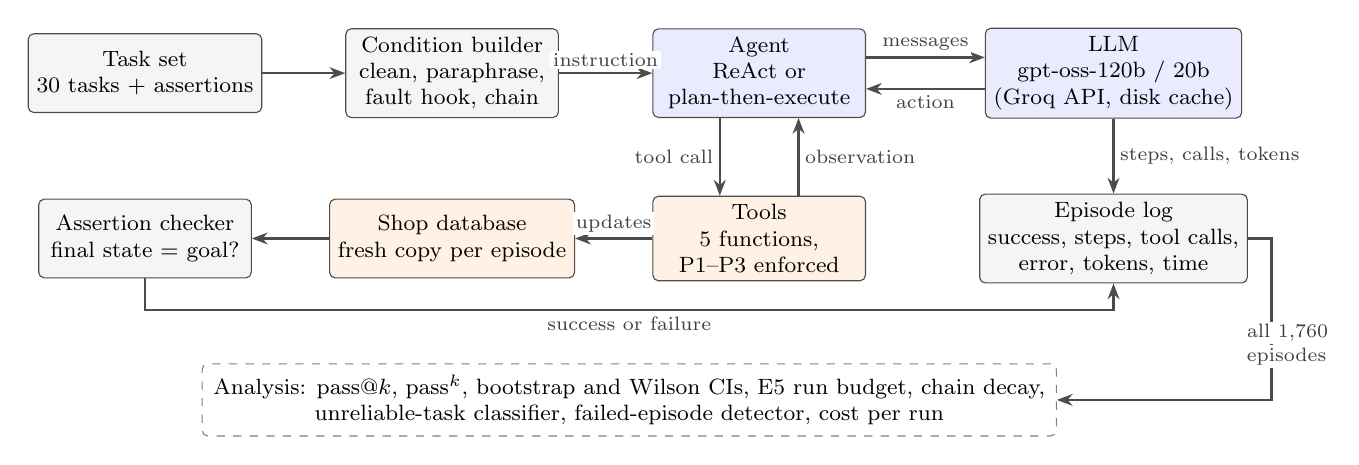
\begin{tikzpicture}[
  box/.style={draw=black!70,rounded corners=2pt,align=center,font=\footnotesize,minimum height=10mm,minimum width=27mm,inner sep=3pt},
  arr/.style={-{Stealth[length=2mm]},thick,black!70},
  lab/.style={font=\scriptsize,black!75,fill=white,inner sep=1pt}]
\node[box,fill=black!4] (tasks) at (0,0) {Task set\\30 tasks + assertions};
\node[box,fill=black!4] (cond) at (3.9,0) {Condition builder\\clean, paraphrase,\\fault hook, chain};
\node[box,fill=blue!8] (agent) at (7.8,0) {Agent\\ReAct or\\plan-then-execute};
\node[box,fill=blue!8] (llm) at (12.3,0) {LLM\\gpt-oss-120b / 20b\\(Groq API, disk cache)};
\node[box,fill=orange!10] (tools) at (7.8,-2.1) {Tools\\5 functions,\\P1--P3 enforced};
\node[box,fill=orange!10] (db) at (3.9,-2.1) {Shop database\\fresh copy per episode};
\node[box,fill=black!4] (check) at (0,-2.1) {Assertion checker\\final state = goal?};
\node[box,fill=black!4] (log) at (12.3,-2.1) {Episode log\\success, steps, tool calls,\\error, tokens, time};
\draw[arr] (tasks) -- (cond);
\draw[arr] (cond) -- node[lab,above=1pt]{instruction} (agent);
\draw[arr] ([yshift=2mm]agent.east) -- node[lab,above=1pt]{messages} ([yshift=2mm]llm.west);
\draw[arr] ([yshift=-2mm]llm.west) -- node[lab,below=1pt]{action} ([yshift=-2mm]agent.east);
\draw[arr] ([xshift=-5mm]agent.south) -- node[lab,left=1pt]{tool call} ([xshift=-5mm]tools.north);
\draw[arr] ([xshift=5mm]tools.north) -- node[lab,right=1pt]{observation} ([xshift=5mm]agent.south);
\draw[arr] (tools) -- node[lab,above=1pt]{updates} (db);
\draw[arr] (db) -- (check);
\draw[arr] (check.south) -- ++(0,-0.4) -| node[lab,pos=0.25,below=1pt]{success or failure} (log.south);
\draw[arr] (llm.south) -- node[lab,right=1pt]{steps, calls, tokens} (log.north);
\node[draw=black!50,dashed,rounded corners=2pt,font=\footnotesize,align=center,inner sep=4pt] (ana) at (6.15,-4.15)
  {Analysis: pass@$k$, $\passk{k}$, bootstrap and Wilson CIs, E5 run budget, chain decay,\\
   unreliable-task classifier, failed-episode detector, cost per run};
\draw[arr] (log.east) -- ++(3mm,0) |- (ana.east);
\node[lab,anchor=west] at (13.95,-3.3) {all 1,760};
\node[lab,anchor=west] at (13.95,-3.6) {episodes};
\end{tikzpicture}
\caption{Evaluation pipeline. The condition builder turns each task into its clean, paraphrased, faulted or chained form;
the fault hook sits between the agent and the tools. Each episode gets a fresh copy of the database, and success is
decided only by the final database state.}\label{fig:pipeline}
\end{figure*}
\subsection{Environment and policies}
The agent acts as customer service for an online electronics shop. The database holds five customers and 12 orders, of
which five are processing, two shipped and five delivered. Five tools are exposed as function calls:
\texttt{lookup\_customer}, \texttt{get\_order}, \texttt{cancel\_order}, \texttt{modify\_order\_address} and
\texttt{refund\_order}, plus \texttt{finish} to end the episode with a reply. The system prompt states four policies:
\begin{enumerate}[label=P\arabic*.,leftmargin=*,itemsep=0pt,topsep=2pt]
\item Cancel or modify an order only while it is processing.
\item Refund only delivered orders, never above the order total.
\item Refunds above 100 must be refused.
\item Act only on orders owned by the customer who is asking.
\end{enumerate}
The tools enforce P1 to P3 and return an error message when a call breaks them. P4 is left to the agent on purpose, so
the wrong-customer tasks test whether the agent refuses on its own.

\subsection{Tasks}
There are 30 tasks in three sets of ten. Each task has an instruction written as a customer message and a list of
assertions on the final database (for example, order O1007 refunded amount equals 100). An episode succeeds when every
assertion holds. For a refusal task the assertions describe the untouched state, so doing nothing correct passes and any
forbidden change fails. Eleven tasks are full refusals and nine have two or more assertions. Every task was solved by
hand against the tools before any model run, and a validator rejects tasks whose assertions are unreachable or already
satisfied when they should not be.

The third set was written to probe edges of the policies: a refund on a shipped order, requests made ``for a friend'' or
``for my neighbour'' on someone else's order, the refund limit from both sides (101 refused, exactly 100 allowed), a
half-order refund that needs a lookup and arithmetic, and multi-step messages where one part must be refused and the
rest carried out.

\subsection{Conditions}
\textbf{Clean.} The task instruction as written.

\textbf{Paraphrase.} Each task has three rewordings (polite, terse, reason-first). A validator checks that every order
id, customer id, amount and address survives exactly and that nothing new is added. Experiments use the first two.

\textbf{Faults.} Before each tool call a fault hook fails the call with probability $\lambda\in\{0.1,0.2\}$. The three
fault types are a timeout, an HTTP 429 rate-limit error and a truncated or garbled payload, chosen with equal
probability. A faulted tool is not executed, so the database is never corrupted and retrying is always safe. The random
stream is seeded from task, seed and rate, and draws exactly three numbers per call, so faults are reproducible.

\textbf{Chains.} A chain joins $L\in\{2,3,4\}$ tasks that touch disjoint orders into one instruction: a short wrapper,
then ``Message 1'', ``Message 2'' and so on, each verbatim. The wrapper says the messages come from separate customers
and that a refusal must not end the conversation. Chain assertions are the union of the member assertions. A
wrong-customer request is never chained with a message from that order's owner, so P4 stays well defined. The step
budget is $15L$. We revised the wrapper wording once. Our first version let the agent end the conversation after a
refusal, because the system prompt tells it to explain a refusal and finish. We reran all chain experiments with the
revised wording, and only those runs are reported.

\begin{algorithm}[t]
\caption{Plan-then-execute with a final action audit}\label{alg:pe}
\small
\begin{algorithmic}[1]
\Require instruction $x$, tools $T$, model $M$, step budget $S$
\State $\mathit{plan}\gets M(\text{planner prompt}, x)$ \Comment{no tools}
\If{$\mathit{plan}$ is empty or a function call} \State ask once more; if still invalid, $\mathit{plan}\gets\varnothing$ \EndIf
\State $\mathit{ledger}\gets[\,]$, $\mathit{audited}\gets$ false
\For{$s=2$ \textbf{to} $S$}
  \State $a\gets M(\text{history};\ \text{system prompt}+\mathit{plan};\ T)$
  \If{$a$ is \texttt{finish}}
    \If{not $\mathit{audited}$}
      \State append \Call{Audit}{$\mathit{ledger}$} to history; $\mathit{audited}\gets$ true; \textbf{continue}
    \EndIf
    \State \Return reply of $a$
  \EndIf
  \State $o\gets T(a)$ \Comment{may be an injected fault}
  \If{$a$ mutates state} append $(a,\ o \text{ starts with OK})$ to $\mathit{ledger}$ \EndIf
  \State append $(a,o)$ to history
\EndFor
\State \Return failure (step budget exhausted)
\end{algorithmic}
\end{algorithm}

\subsection{Agents}
\textbf{ReAct}~\cite{react} runs a loop of model reply, one tool call and one observation until the model calls
\texttt{finish}, the step budget runs out, or three replies in a row cannot be parsed.

\textbf{Plan-then-execute with audit} (Algorithm~\ref{alg:pe}) first asks for a short numbered plan, then runs the same
ReAct loop with the plan appended to the system prompt. It keeps a ledger of every mutating call and whether the tool
confirmed it. The first time the model calls \texttt{finish}, the agent does not stop. It sends one message listing the
confirmed and rejected actions and asks the model to finish only if every request has been handled. The second
\texttt{finish} ends the episode. The audit is built from tool outputs, so it cannot repeat a hallucinated action back to
the model.

The planning step needed two fixes, and every plan-then-execute result in this paper comes from the fixed version. In
our first runs the planner reused the executor's ``call a function'' prompt with tools switched off. gpt-oss tried to call
a tool anyway, the API rejected the reply, and most episodes ran with no plan or with a raw tool call pasted in as the
plan. The planner now has its own prompt, which lists the policies and tools for reference only, and its reply is
checked: an empty reply or one that looks like a function call is rejected and asked for once more. After that fix the
plans were valid text but guessed facts the planner had not seen, such as who owns an order or its total, and sometimes
wrote the final reply in advance; the executor followed those guesses and skipped \texttt{get\_order}. The planner is
now told that it has seen no order data, and each step must read ``\texttt{get\_order}, then ACT only if the owner,
status and limits allow it, otherwise REFUSE'', with no decided outcome and no pre-written reply. Every episode logs
whether it got a valid plan (\texttt{plan\_ok}); all 180 plan-then-execute episodes did. Results from the earlier
planner versions were discarded.

\subsection{Models and settings}
Both models are the open-weight gpt-oss family~\cite{gptoss}, served through the Groq API with temperature 0.7 and
reasoning effort set to low. The clean ReAct runs (E1) and all plan-then-execute runs used seeds 0 to 4. The ReAct runs
of E2 to E4 used seeds 0 to 9. Every successful reply is cached on disk under a hash of messages, model, temperature,
seed, tools and reasoning effort, so interrupted runs resume without new calls and re-runs are exact. Failed API calls
are never cached. Episodes that ended in an API error or a crash are dropped from all metrics instead of being counted
as task failures. From the plan-then-execute reruns on, every log row also records prompt and completion tokens,
wall-clock time, API calls and cache hits. As a pilot for a third model family, qwen3.8-27b ran three tasks with both
agents through the same client, tools and policies. Fig.~\ref{fig:pipeline} shows the pipeline.

\section{Metrics and Analysis Methods}
\subsection{Success metrics}
A unit is a task (or a task with one paraphrase, or a chain) under one agent, model and condition. With $n$ runs and $c$
successes, we report
\begin{equation}
\passat{1}=\frac{c}{n},\quad
\passat{k}=1-\frac{\binom{n-c}{k}}{\binom{n}{k}},\quad
\passk{k}=\frac{\binom{c}{k}}{\binom{n}{k}},
\end{equation}
averaged over units. pass@$k$ is the chance that at least one of $k$ runs succeeds~\cite{codex}; $\passk{k}$ is the
chance that all $k$ succeed~\cite{taubench}. Both are unbiased for $k\le n$, so $\passk{5}$ is comparable between units
with five and with ten runs, and the ten-run units are estimated more precisely. Paraphrases of the same task are
separate units, never pooled.

\subsection{Confidence intervals}
Runs of one task are correlated, so we resample tasks, not episodes. With eight or more task clusters we use a cluster
bootstrap (4,000 resamples, 95\% percentile interval). With fewer clusters, or when every bootstrap resample is
identical, we use a Wilson interval~\cite{wilson} with $n$ equal to the number of tasks or chains. Most intervals are
wide, and we report them.

\subsection{Run budget (E5)}
To ask how many runs are enough, we score every subset of $n'$ of the ten seeds ($\binom{10}{n'}$ subsets) and compare
with the full data in two ways: (a) the share of subsets in which the 120b-versus-20b ordering on pass@1 is reversed or
tied, per condition; (b) the Kendall $\tau_b$~\cite{kendall} between the ranking of all agent-model-condition cells from
the subset and from all ten runs. Only cells that have all ten runs enter (b).

\subsection{Chain decay}
If each message in a chain of length $L$ succeeded independently with the single-task rate $p$, the chain would succeed
with $p^L$. We compare observed chain success $\hat q_L$ to $p^L$, where $p$ is the clean pass@1 pooled over all 30
tasks, and report the implied per-message success $\hat q_L^{1/L}$ with its interval transformed the same way.

\subsection{Predicting unreliable tasks}
We label a unit unreliable if any of its runs failed ($\passk{n}<1$). Features are the run setting (model, agent,
paraphrase flag, fault rate, chain length) and task descriptors computed from the task file: number of requests, orders
and state-changing requests, refusal parts, wrong-customer and social-pressure cues, refunds near the limit, whether a
lookup is needed, and length. Chains sum or take the maximum over members. We fit logistic regression and gradient
boosting (scikit-learn~\cite{sklearn}) and evaluate by leave-one-task-out: when a single task is held out, every chain
containing it is removed from training too. AUC intervals bootstrap the held-out tasks.

\begin{table}[t]
\caption{Experiments and valid episodes after removing API errors}\label{tab:exp}
\centering\small
\begin{tabular}{@{}llll@{}}
\toprule
Exp. & What varies & Units & Episodes\\
\midrule
E1 & clean (P\&E: set 2 only) & 30 tasks & 300 + 100\\
E2 & two paraphrases (set 2) & 10 tasks & 400\\
E3 & fault rate 0.1 and 0.2 (set 2) & 10 tasks & 400\\
E4 & chains, $L=2,3,4$ & 8 per $L$ & 480 + 80\\
E5 & seed subsets of E2--E4 & 12 cells & (reuse)\\
\midrule
\multicolumn{3}{@{}l}{Total} & 1,760\\
\bottomrule
\end{tabular}

\smallskip
\footnotesize Second numbers are plan-then-execute episodes (P\&E chains: four chains each of $L=2$ and $L=4$, five runs).
ReAct runs of E2--E4 have ten runs per unit, E1 five. Chains are built from sets 1 and 2.
\end{table}

\subsection{Detecting failed episodes}
A second model predicts whether a single episode failed, using the run setting plus trace features: steps, tool calls,
calls per step, and steps and calls per chain message. Latency is excluded because cached replays take almost no time.
Evaluation is again leave-one-task-out.

\section{Experiments}
Table~\ref{tab:exp} lists the five experiments. Each one answers a single question, and each stress condition is
compared against a clean baseline on the same tasks. This section gives the protocol shared by all runs, then the setup
of each experiment.

\subsection{Run protocol}
The runners loop over seeds in the outer loop, so if a run is cut off, the completed part is still balanced across
tasks. We ran one worker with a one-second pause between episodes to stay under the API rate limit. Each finished
episode is appended to a JSONL log with the task, agent, model, condition, seed, success flag, step count, tool-call
count, error field and latency. A runner that is stopped and restarted skips every episode already in its log and
retries only those that ended in an API error or a crash, and the merge step keeps one record per episode and only units
with all their runs.

The step budget was 15 for single tasks and $15L$ for a chain of length $L$, so a long chain cannot fail on the step cap
alone. In practice no valid episode reached the cap, and only one, a plan-then-execute chain that had already made the
right changes, ended on the limit of three unparseable replies. Every failure we report is an episode in which the agent
called \texttt{finish} and left the database in the wrong state.

The runners logged 1,770 episode records in the files used here. Ten ended in an API error, mostly after the daily token
limit was reached, and were dropped, leaving the 1,760 valid episodes used in all analyses.

\subsection{E1: clean baseline}
E1 measures each model with ReAct on all 30 tasks, unchanged: $30\times2\times5=300$ episodes. It is the reference for
the other experiments and the input to the chain-decay prediction. We also ran plan-then-execute on the ten set-2 tasks
($10\times2\times5=100$ episodes), which is the set used by E2 and E3, so the two agents can be compared on the same
tasks.



\subsection{E2: paraphrase robustness}
E2 asks whether rewording a request changes the outcome. Each set-2 task has three hand-written paraphrases, and E2 uses
the first two: 10 tasks $\times$ 2 $\times$ 2 models $\times$ 10 runs $=$ 400 episodes. Each paraphrase is its own unit,
so a model that handles one wording and fails the other is not averaged into a single score. The paraphrase validator
guarantees that every id, amount and address is unchanged, so any difference in outcome comes from the wording alone.

\subsection{E3: tool faults}
E3 runs the set-2 tasks with fault rates $\lambda=0.1$ and $0.2$: $10\times2\times2\times10=400$ episodes. With about
two to three tool calls per episode (Table~\ref{tab:effort}), a rate of 0.2 means that about four episodes in ten see at
least one failed call. Faults are transient and the database is never touched, so a careful agent can always recover by
reading the error and retrying. E3 therefore tests error handling, not luck. Because the fault stream is seeded per
task, seed and rate, the two models face the same fault pattern for the same number of calls.

\subsection{E4: request chains}
The chain builder produced a frozen file of 30 chains, ten each of length 2, 3 and 4, from the 20 tasks in sets 1 and 2
with a fixed seed. It balances how often each task is used and never combines tasks that share an order. ReAct ran the
first eight chains of each length with ten runs: $8\times3\times2\times10=480$ episodes. The chain ids are frozen in a
list so that every later run uses exactly the same chains. Between them the chains mix ordinary requests, refusals and
wrong-customer requests, so a correct run needs both actions and refusals in one conversation. Plan-then-execute ran the
first four chains of lengths 2 and 4 with five runs ($4\times2\times2\times5=80$ episodes), paired with the ReAct runs on
the same chains and seeds. A later run of the first four length-3 chains is reported in Section~\ref{sec:pe} from its
summary only.

\subsection{E5: run budget}
E5 needs no new runs. It resamples the seeds of E2 to E4 as described in Section~\ref{sec:e5res}, over the 12 ReAct cells
(model and condition) that have all ten runs.

\subsection{Agent effort per condition}
Table~\ref{tab:effort} gives the mean number of steps and tool calls per episode. Faults add a fraction of a call per
episode, which is the retries. The chain rows are the more telling ones. A four-request chain needs at least one call
per request, yet ReAct with gpt-oss-20b made 2.5 tool calls on average and gpt-oss-120b made 4.0, against 7.5 to 8.0 for
plan-then-execute. These counts already point at the premature-finish failure analysed in Section~\ref{sec:chains}.

\begin{table}[t]
\caption{Mean steps and tool calls per valid episode}\label{tab:effort}
\centering\small
\begin{tabular}{@{}llrrr@{}}
\toprule
Agent & Condition & Episodes & Steps & Tool calls\\
\midrule
\multirow{7}{*}{ReAct, 120b} & clean (30 tasks) & 150 & 3.1 & 2.1\\
 & paraphrase & 200 & 3.1 & 2.0\\
 & faults $\lambda=0.1$ & 100 & 3.3 & 2.3\\
 & faults $\lambda=0.2$ & 100 & 3.6 & 2.5\\
 & chains $L=2$ & 80 & 5.2 & 4.1\\
 & chains $L=3$ & 80 & 7.1 & 5.9\\
 & chains $L=4$ & 80 & 5.2 & 4.0\\
\midrule
\multirow{7}{*}{ReAct, 20b} & clean (30 tasks) & 150 & 3.0 & 2.0\\
 & paraphrase & 200 & 3.0 & 2.0\\
 & faults $\lambda=0.1$ & 100 & 3.2 & 2.2\\
 & faults $\lambda=0.2$ & 100 & 3.2 & 2.2\\
 & chains $L=2$ & 80 & 4.5 & 3.4\\
 & chains $L=3$ & 80 & 6.1 & 5.1\\
 & chains $L=4$ & 80 & 3.5 & 2.5\\
\midrule
\multirow{3}{*}{P\&E, 120b} & clean (set 2) & 50 & 5.2 & 2.1\\
 & chains $L=2$ & 20 & 8.2 & 4.5\\
 & chains $L=4$ & 20 & 11.6 & 8.0\\
\midrule
\multirow{3}{*}{P\&E, 20b} & clean (set 2) & 50 & 5.2 & 2.2\\
 & chains $L=2$ & 20 & 7.7 & 4.5\\
 & chains $L=4$ & 20 & 10.7 & 7.5\\
\bottomrule
\end{tabular}

\smallskip
\footnotesize Steps count every model call, so plan-then-execute adds the plan call and the audit turn.
\end{table}

\subsection{Budget}
The free Groq tier allows 8,000 tokens per minute and 200,000 tokens per model per day, and chain episodes use several
times more tokens than single tasks because the whole conversation is resent at every step. A four-request
plan-then-execute chain used about 22,000 tokens (Table~\ref{tab:cost}), so one key allowed only eight or nine of them
per model per day. The full design (three paraphrases on all 30 tasks, ten chains per length, ten runs everywhere) was
out of reach. We ran on several accounts over several days and cut the number of tasks and chains before the number of
runs. E1 and the plan-then-execute runs stayed at five runs.

\section{Results}
\subsection{Clean baseline}
Without any disturbance ReAct reaches pass@1 0.993 ($\passk{5}$ 0.967) with gpt-oss-120b and 0.913 ($\passk{5}$ 0.867)
with gpt-oss-20b over the 30 tasks. Table~\ref{tab:sets} splits this by task set. Sets 1 and 2 are near ceiling for both
models, and the edge-case tasks in set 3 are where the models separate. The 20b model failed three of them: the refund
of exactly 100 (3 of 5 runs), a cancel of a shipped order combined with an address change (4 of 5), and a full refund
plus an extra ``goodwill'' amount that must be refused (5 of 5). In the first case it refused a legal request; in the
last two it carried out a part it should have refused, or failed to finish the allowed part.

\begin{table}[t]
\caption{Clean ReAct results by task set}\label{tab:sets}
\centering\small
\begin{tabular}{@{}lccccc@{}}
\toprule
 & \multicolumn{3}{c}{pass@1} & Set 3 & Failed\\
\cmidrule(lr){2-4}
Model & Set 1 & Set 2 & Set 3 & $\passk{5}$ & set-3 tasks\\
\midrule
120b & 1.00 & 1.00 & 0.98 & 0.90 & 1\\
20b & 0.98 & 1.00 & 0.76 & 0.70 & 3\\
\bottomrule
\end{tabular}
\end{table}

\begin{table}[t]
\caption{ReAct on set 2 under paraphrases and tool faults}\label{tab:stress}
\centering\small
\setlength{\tabcolsep}{4pt}
\begin{tabular}{@{}lcccccc@{}}
\toprule
 & \multicolumn{3}{c}{gpt-oss-120b} & \multicolumn{3}{c}{gpt-oss-20b}\\
\cmidrule(lr){2-4}\cmidrule(lr){5-7}
Condition & pass@1 & $\passk{5}$ & $\passk{10}$ & pass@1 & $\passk{5}$ & $\passk{10}$\\
\midrule
Clean & 1.00 & 1.00 & -- & 1.00 & 1.00 & --\\
Paraphrase & 0.95 & 0.93 & 0.90 & 0.96 & 0.84 & 0.80\\
Faults $\lambda=0.1$ & 0.98 & 0.92 & 0.90 & 0.94 & 0.72 & 0.50\\
Faults $\lambda=0.2$ & 0.94 & 0.77 & 0.70 & 0.81 & 0.46 & 0.40\\
\bottomrule
\end{tabular}

\smallskip
\footnotesize 10 tasks (20 paraphrase units), 10 runs each; clean has 5 runs. 95\% interval of $\passk{5}$ at
$\lambda=0.2$: 0.53--1.00 (120b), 0.18--0.75 (20b).
\end{table}

\subsection{pass@1 versus $\passk{k}$ under paraphrases and faults}
Table~\ref{tab:stress} and Fig.~\ref{fig:bars} compare each stress condition with its own clean baseline, the second
task set, on which both models score 1.00. Rewording mattered little for single runs (pass@1 0.95 and 0.96), but with
ten runs it shows up in reliability: two of the 20 paraphrase units failed at least once for gpt-oss-120b and four for
gpt-oss-20b. Faults mattered more, and mostly in $\passk{k}$. At $\lambda=0.2$ the 20b model still succeeds on 81\% of
single runs, but only 40\% of the tasks succeed in all ten. The 120b model keeps pass@1 at 0.94 and drops to 0.70 on
$\passk{10}$. Fig.~\ref{fig:passk} shows $\passk{k}$ for $k=1$ to 10: under faults the 20b curves keep falling as $k$
grows, while the clean and paraphrase curves stay almost flat. Five runs would have hidden part of this: at
$\lambda=0.1$ the 20b model's $\passk{5}$ is 0.72 and its $\passk{10}$ is 0.50.

\begin{figure*}[t]
\centering
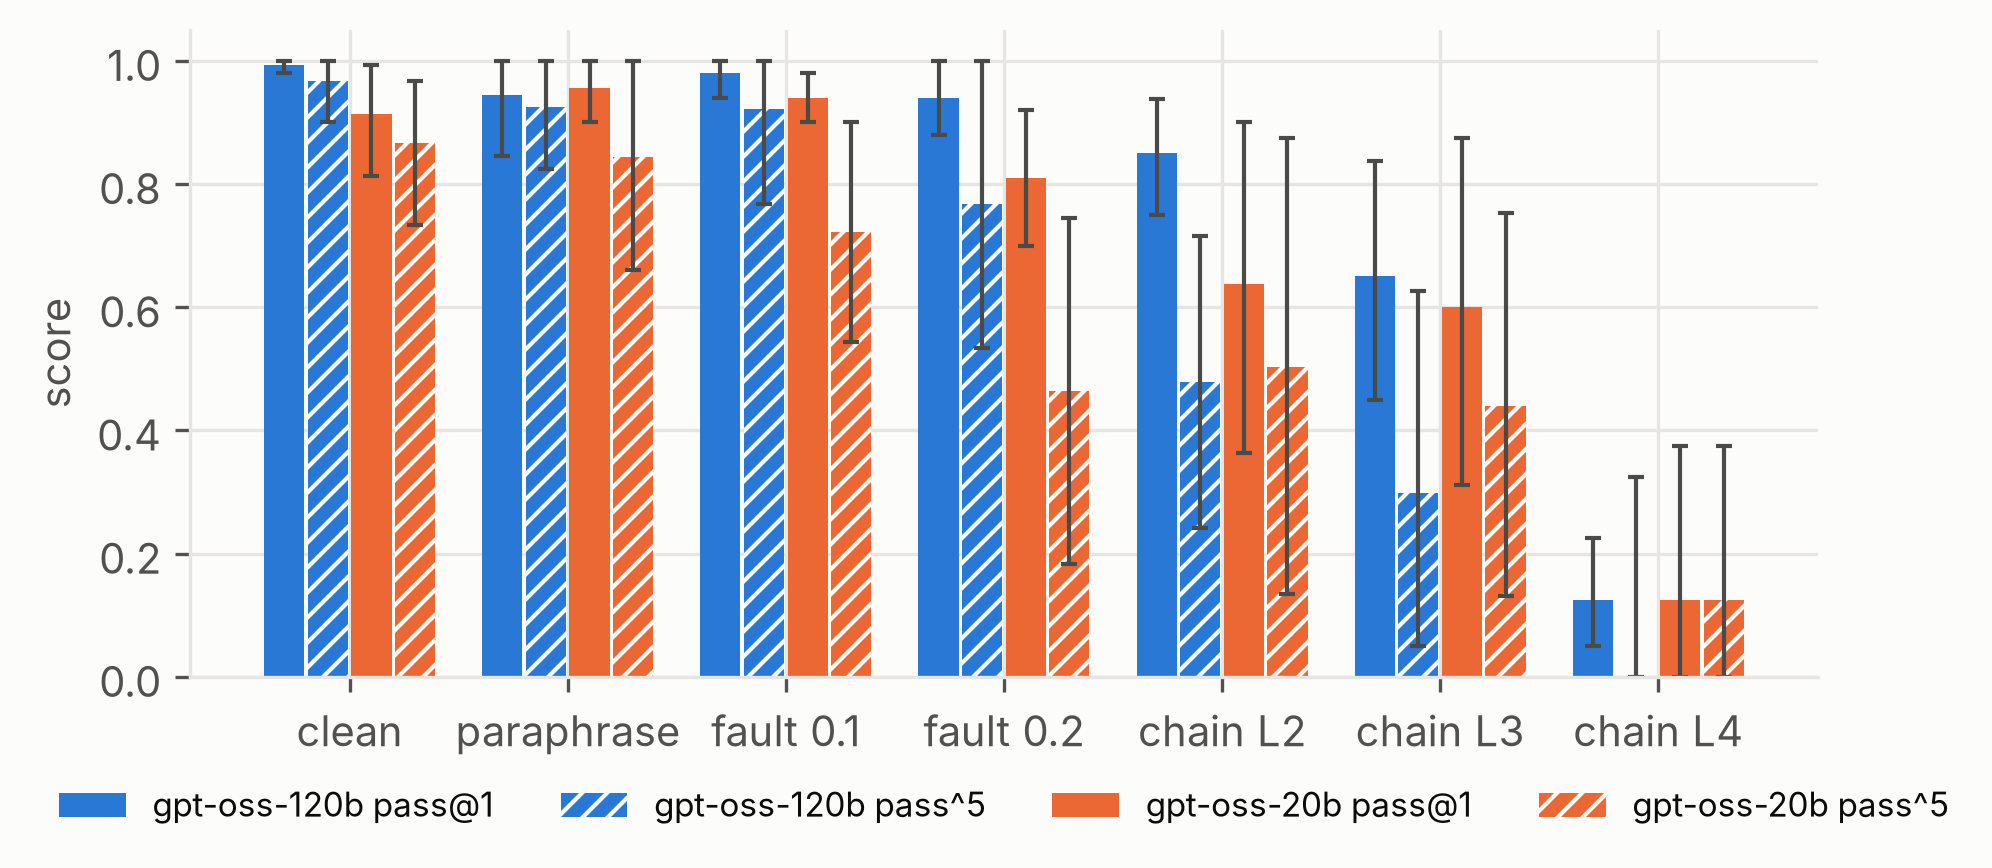
\includegraphics[width=0.78\textwidth]{fig2_bars.png}
\caption{ReAct pass@1 (solid) and $\passk{5}$ (hatched) per condition with 95\% intervals. Clean bars use all 30 tasks;
paraphrase and fault bars use set 2; chains use eight chains per length.}\label{fig:bars}
\end{figure*}

\begin{figure*}[t]
\centering
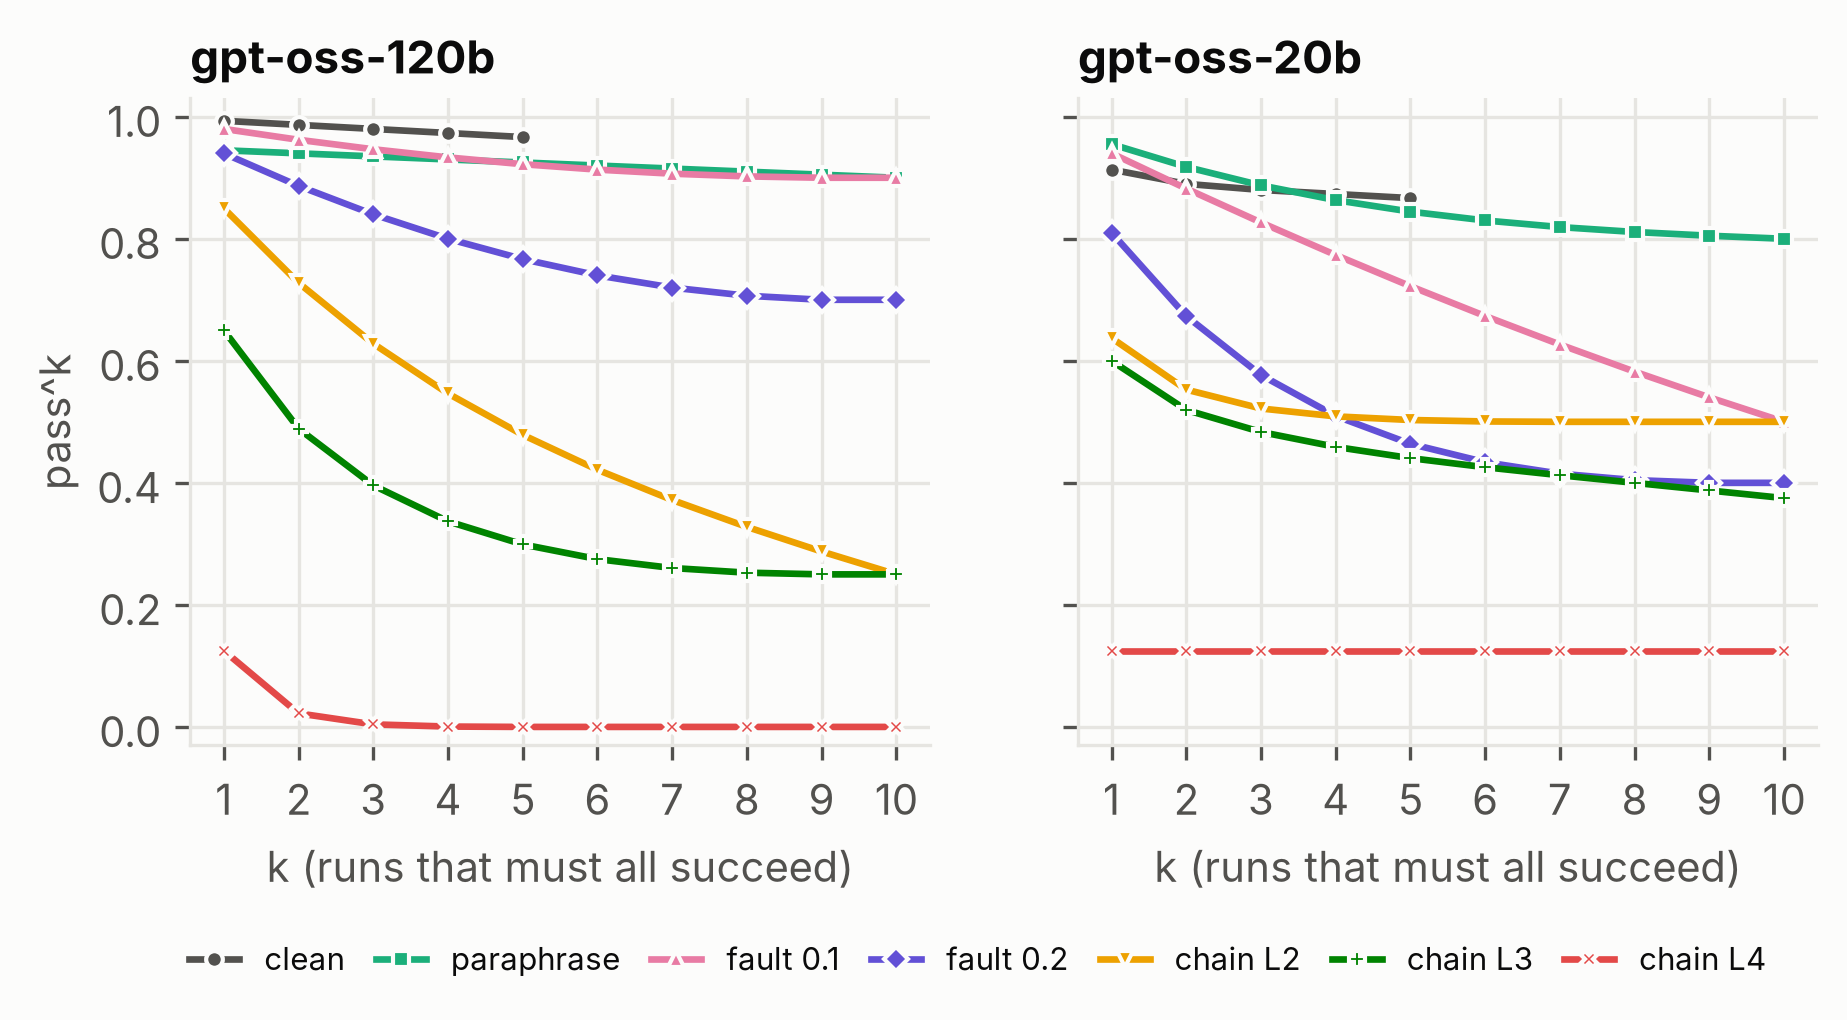
\includegraphics[width=0.78\textwidth]{fig3_passk.png}
\caption{ReAct $\passk{k}$ as $k$ grows (clean has five runs, so it stops at $k=5$). Under faults the 20b model loses
reliability with every extra required run, and four-request chains sit at or near zero for both models.}\label{fig:passk}
\end{figure*}

\subsection{Chains}\label{sec:chains}
Chains were the clearest failure (Table~\ref{tab:chain}, Fig.~\ref{fig:chain}). The 120b model went from 0.99 on single
tasks to 0.85, 0.65 and 0.13 on chains of two, three and four requests. Under independent errors the four-request
prediction is 0.97. The 20b model reached 0.64, 0.60 and 0.13. Its two- and three-request numbers are within noise of
each other: each length uses different chains built from different tasks, so the step from $L=2$ to $L=3$ mixes chain
length with task difficulty. The implied per-message success for 120b drops from 0.99 to 0.92, 0.87 and 0.60 as $L$
grows, so each message becomes harder to handle the longer the conversation is. The prediction is, if anything, generous
to the models: the pooled $p$ includes the hard set-3 tasks, which never appear in chains.

\begin{table}[t]
\caption{Chain success against the independent-errors prediction (ReAct)}\label{tab:chain}
\centering\small
\setlength{\tabcolsep}{4pt}
\begin{tabular}{@{}llcccc@{}}
\toprule
Model & $L$ & Observed & $p^L$ & Implied $\hat q^{1/L}$ & 95\% CI (implied)\\
\midrule
\multirow{4}{*}{120b} & 1 & 0.993 & 0.993 & 0.993 & 0.875--1.000\\
 & 2 & 0.850 & 0.987 & 0.922 & 0.710--0.984\\
 & 3 & 0.650 & 0.980 & 0.866 & 0.688--0.957\\
 & 4 & 0.125 & 0.974 & 0.595 & 0.385--0.828\\
\midrule
\multirow{4}{*}{20b} & 1 & 0.913 & 0.913 & 0.913 & 0.761--0.972\\
 & 2 & 0.637 & 0.834 & 0.798 & 0.561--0.933\\
 & 3 & 0.600 & 0.762 & 0.843 & 0.660--0.947\\
 & 4 & 0.125 & 0.696 & 0.595 & 0.385--0.828\\
\bottomrule
\end{tabular}

\smallskip
\footnotesize $L=1$: 150 clean episodes per model. $L\ge2$: 8 chains $\times$ 10 runs.
\end{table}

Reading the failed traces showed a consistent pattern. On four-request chains the agent usually called \texttt{finish}
after one to three tool calls and wrote a reply that described actions it never took, sometimes citing policies that do
not exist. This is a premature-termination failure, not a slow drift of small errors, and it is why the
independent-errors model is so far off.

\begin{figure*}[t]
\centering
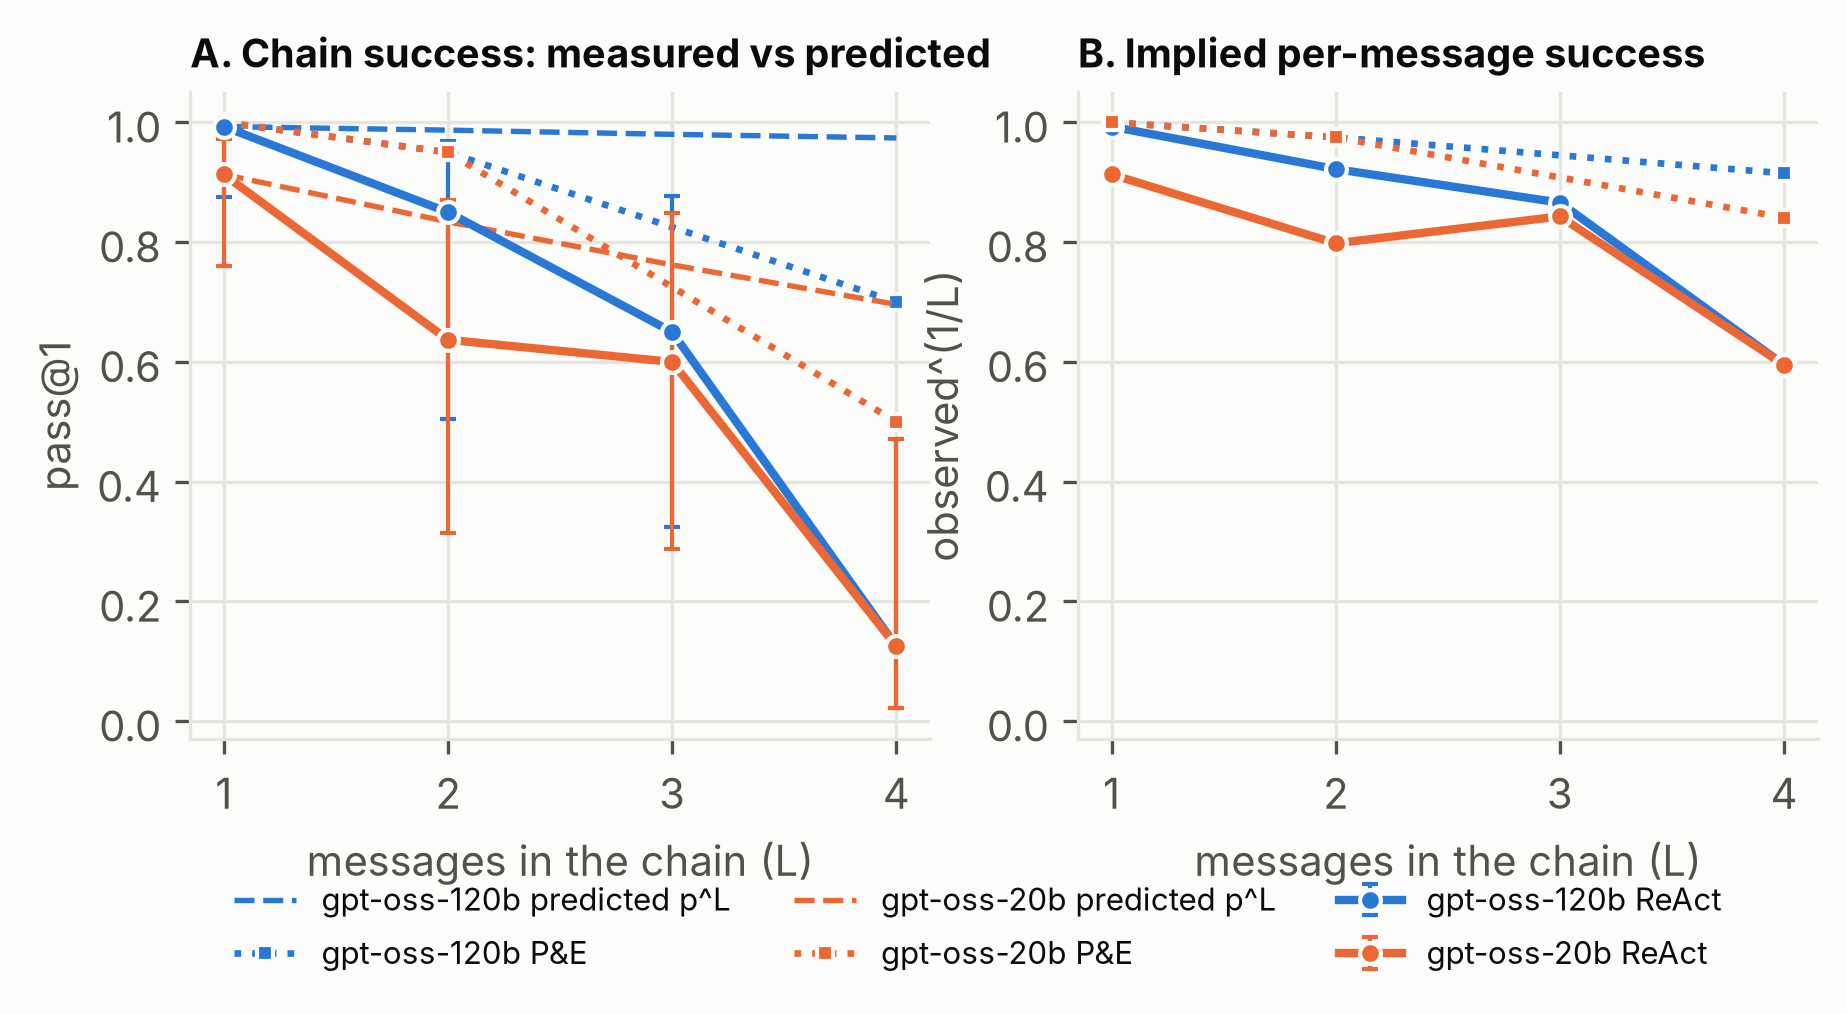
\includegraphics[width=0.72\textwidth]{fig4_chain.png}
\caption{Chain decay. Left: measured chain success against $p^L$ (dashed), for ReAct (solid, eight chains, ten runs) and
plan-then-execute (dotted, four chains of $L=2$ and $L=4$, five runs). Right: implied per-message success
$\hat q_L^{1/L}$, which should stay flat if messages failed independently.}\label{fig:chain}
\end{figure*}

\subsection{Plan-then-execute}\label{sec:pe}
Table~\ref{tab:pe} compares the two agents on the same tasks, chains and seeds (0 to 4). On single tasks both are
perfect. On two-request chains plan-then-execute is a little better for 120b and clearly better for 20b (0.95 against
0.50), though with four chains the 20b interval still includes zero. On four-request chains the difference is large for
both models: 0.70 against 0.05 for 120b, a paired difference of $+0.65$ (95\% CI 0.45 to 0.90 over four chains), and
0.50 against 0.00 for 20b ($+0.50$, CI 0.15 to 0.85). Reliability across runs improves less. $\passk{5}$ on four-request
chains rises only from 0.00 to 0.25 for both models, because one of the four chains succeeds every time and the others
only sometimes. Eight of the 20b model's ten failures came from the two chains that contain A10 (``refund the full
amount''), where it reads a full refund as exceeding the order total.

\begin{table}[t]
\caption{ReAct versus plan-then-execute on the same units and seeds (pass@1 unless noted)}\label{tab:pe}
\centering\small
\setlength{\tabcolsep}{4pt}
\begin{tabular}{@{}lcccc@{}}
\toprule
 & \multicolumn{2}{c}{gpt-oss-120b} & \multicolumn{2}{c}{gpt-oss-20b}\\
\cmidrule(lr){2-3}\cmidrule(lr){4-5}
Setting & ReAct & P\&E & ReAct & P\&E\\
\midrule
Set 2, single & 1.00 & 1.00 & 1.00 & 1.00\\
Set 2, single, $\passk{5}$ & 1.00 & 1.00 & 1.00 & 1.00\\
Chains $L=2$ & 0.90 & 0.95 & 0.50 & 0.95\\
Chains $L=3$$^{\ast}$ & 0.85 & 0.80 & 0.80 & 0.75\\
Chains $L=4$ & 0.05 & 0.70 & 0.00 & 0.50\\
Chains $L=4$, $\passk{5}$ & 0.00 & 0.25 & 0.00 & 0.25\\
\bottomrule
\end{tabular}

\smallskip
\footnotesize Four chains per length, five runs (seeds 0--4) for both agents; ReAct is cut to the same seeds.
Paired differences at $L=2$: $+0.05$ (CI 0.00--0.15, 120b), $+0.45$ ($-0.10$--1.00, 20b).
$^{\ast}$Later run, summary only; not included in the other analyses.
\end{table}

Three-request chains did not follow this pattern. On the first four length-3 chains, plan-then-execute scored 0.80 and
0.75 against 0.85 and 0.80 for ReAct, so no gain, with every chain solved at least once by both agents. These four
chains are easier for ReAct than the full set of eight (0.85 against 0.65 for 120b), which leaves less room to improve,
and four chains cannot separate a small loss from noise. We therefore read the plan-then-execute result as a large gain
on the longest chains, where ReAct's early finish dominates, and no measurable effect elsewhere. We could not run the
ablation that would separate the plan from the audit.

\subsection{Cost per run}
Table~\ref{tab:cost} uses the token fields logged from the plan-then-execute reruns on. Cost roughly doubles with each
step up in chain length, because every step resends the whole conversation: about 5,600 tokens for a single task, 11,000
to 12,000 for two requests and 21,000 to 24,000 for four. Per successful episode the four-request chains cost 34,000
(120b) and 42,000 (20b) tokens. The ReAct runs predate token logging; in the pilot, ReAct used 2,400 to 3,300 tokens per
single task with gpt-oss, so the plan and audit roughly double the cost of a single task. qwen3.8-27b solved all three
pilot tasks with both agents (six episodes) at about 4,400 (ReAct) and 8,600 (plan-then-execute) tokens per episode.

\begin{table}[t]
\caption{Plan-then-execute cost per episode}\label{tab:cost}
\centering\small
\setlength{\tabcolsep}{3.5pt}
\begin{tabular}{@{}llrrrrr@{}}
\toprule
Model & Setting & Tokens & Calls & Time (s) & Tok./success & Per key\\
\midrule
\multirow{3}{*}{120b} & single & 5,670 & 5.2 & 20 & 5,670 & 35\\
 & $L=2$ & 12,094 & 8.2 & 87 & 12,730 & 16\\
 & $L=4$ & 24,077 & 11.6 & 248 & 34,396 & 8\\
\midrule
\multirow{3}{*}{20b} & single & 5,520 & 5.2 & 14 & 5,520 & 36\\
 & $L=2$ & 11,114 & 7.6 & 103 & 11,699 & 17\\
 & $L=4$ & 21,163 & 10.6 & 241 & 42,327 & 9\\
\bottomrule
\end{tabular}

\smallskip
\footnotesize Means per episode. ``Per key'': episodes that fit in one free-tier day (200,000 tokens per model). Time is
wall clock, including rate-limit waits.
\end{table}

\subsection{How many runs are enough?}\label{sec:e5res}
Table~\ref{tab:e5} and Fig.~\ref{fig:budget} summarise the run-budget analysis over the 12 ReAct cells that have all ten
runs. The mean agreement with the full-data ranking reaches Kendall $\tau_b=0.90$ at five runs, but the worst subset
reaches 0.9 only at nine runs. Pairwise comparisons are more fragile. With one run, the 120b-versus-20b ordering was
reversed or tied in 60\% of subsets for paraphrases, for faults at 0.1 and for three-request chains, 30\% for two-request
chains and 20\% for faults at 0.2. At three runs faults at 0.2 never flipped and two-request chains almost never (3\%),
but three-request chains still flipped in 39\% and paraphrases in 49\%. Paraphrases are a near tie at full data (0.95
against 0.96), so no affordable number of runs settles their order. Four-request chains are an exact tie at full data
and are left out of (a). Clean runs never flipped.

\begin{table}[t]
\caption{Ranking stability against the number of runs per task}\label{tab:e5}
\centering\small
\begin{tabular}{@{}rrccc@{}}
\toprule
Runs & Subsets & Mean $\tau_b$ & Worst $\tau_b$ & Worst $\ge0.9$\\
\midrule
1 & 10 & 0.76 & 0.53 & no\\
2 & 45 & 0.84 & 0.69 & no\\
3 & 120 & 0.86 & 0.70 & no\\
4 & 210 & 0.89 & 0.73 & no\\
5 & 252 & 0.90 & 0.77 & no\\
6 & 210 & 0.92 & 0.81 & no\\
7 & 120 & 0.93 & 0.81 & no\\
8 & 45 & 0.95 & 0.86 & no\\
9 & 10 & 0.97 & 0.90 & just\\
10 & 1 & 1.00 & 1.00 & yes\\
\bottomrule
\end{tabular}

\smallskip
\footnotesize 12 cells: two models $\times$ paraphrase, two fault rates and three chain lengths. Worst $\tau_b$ at nine
runs is 0.898.
\end{table}

\begin{figure*}[t]
\centering
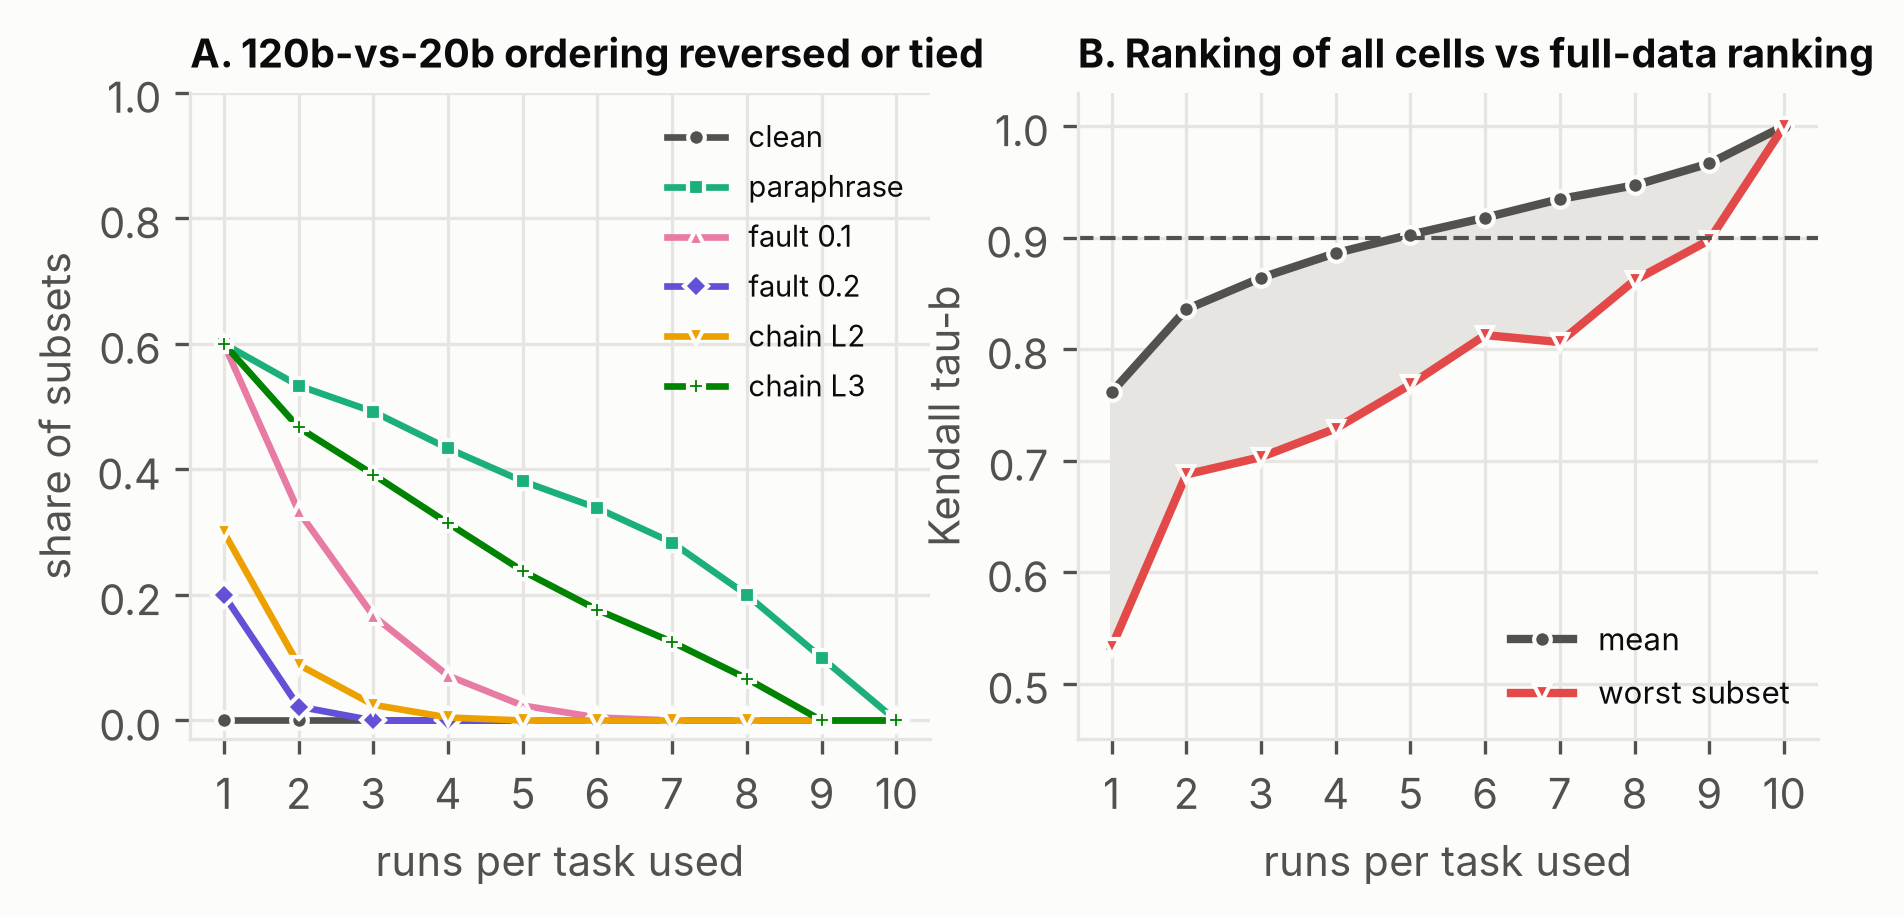
\includegraphics[width=0.72\textwidth]{fig5_budget.png}
\caption{Run budget. Left: share of seed subsets in which the 120b-versus-20b ordering is reversed or tied (clean has
five runs). Right: Kendall $\tau_b$ between subset and full-data rankings of all ten-run cells (mean and worst
subset).}\label{fig:budget}
\end{figure*}

\subsection{Which tasks are unreliable?}
Of 224 units, 70 are unreliable. Table~\ref{tab:clf} gives leave-one-task-out AUCs. The run setting alone carries almost
no signal across tasks (0.49 for gradient boosting), because most settings contain both reliable and unreliable tasks.
Adding task descriptors raises AUC to 0.88 overall, 0.84 on single tasks and 0.77 on chains. The logistic coefficients
point the same way as the results above (longer chains, higher fault rates and more state-changing requests raise risk;
the 120b model and plan-then-execute lower it), but with 70 positives we do not read individual weights. One caution:
a unit with ten runs has more chances to fail once than a unit with five, so the label is stricter for the E2 to E4
units than for E1 and plan-then-execute. Fig.~\ref{fig:clf} shows all four model and feature combinations.

\begin{table}[t]
\caption{Unreliable-task classifier, leave-one-task-out AUC}\label{tab:clf}
\centering\small
\begin{tabular}{@{}llccc@{}}
\toprule
Units & Model & Setting & + task & 95\% CI (+ task)\\
\midrule
All (224) & boosting & 0.49 & 0.88 & 0.83--0.93\\
All (224) & logistic & 0.54 & 0.84 & 0.78--0.90\\
Single (160) & boosting & 0.56 & 0.84 & 0.77--0.92\\
Chains (64) & boosting & 0.36 & 0.77 & 0.64--0.87\\
\bottomrule
\end{tabular}
\end{table}

\begin{table}[t]
\caption{Failed-episode detector, leave-one-task-out AUC}\label{tab:det}
\centering\small
\begin{tabular}{@{}llccc@{}}
\toprule
Episodes & Model & Setting & + trace & 95\% CI (+ trace)\\
\midrule
All (1,760) & logistic & 0.85 & 0.86 & 0.78--0.91\\
Single (1,200) & logistic & 0.57 & 0.60 & 0.47--0.76\\
Chains (560) & logistic & 0.77 & 0.85 & 0.77--0.91\\
Chains (560) & boosting & 0.71 & 0.81 & 0.69--0.89\\
\bottomrule
\end{tabular}
\end{table}

\subsection{Detecting failed episodes}
The episode-level detector (Table~\ref{tab:det}, Fig.~\ref{fig:det}) reaches AUC 0.86 over all 1,760 episodes, but most
of that comes from chain length, since chains fail far more often. On single tasks, where only 67 of 1,200 episodes
failed, trace features add little and the interval reaches chance. On chains they help: AUC rises from 0.77 to 0.85 for
logistic regression. A failed chain has few tool calls per message, which matches the premature-finish pattern. The gain
is smaller than the 0.87 to 0.97 we saw on the first 91 chain episodes, so the earlier number was optimistic. This makes
the detector a post-hoc check on a finished run, useful for flagging replies before they reach a customer, but not an
early warning.

\begin{figure}[t]
\centering
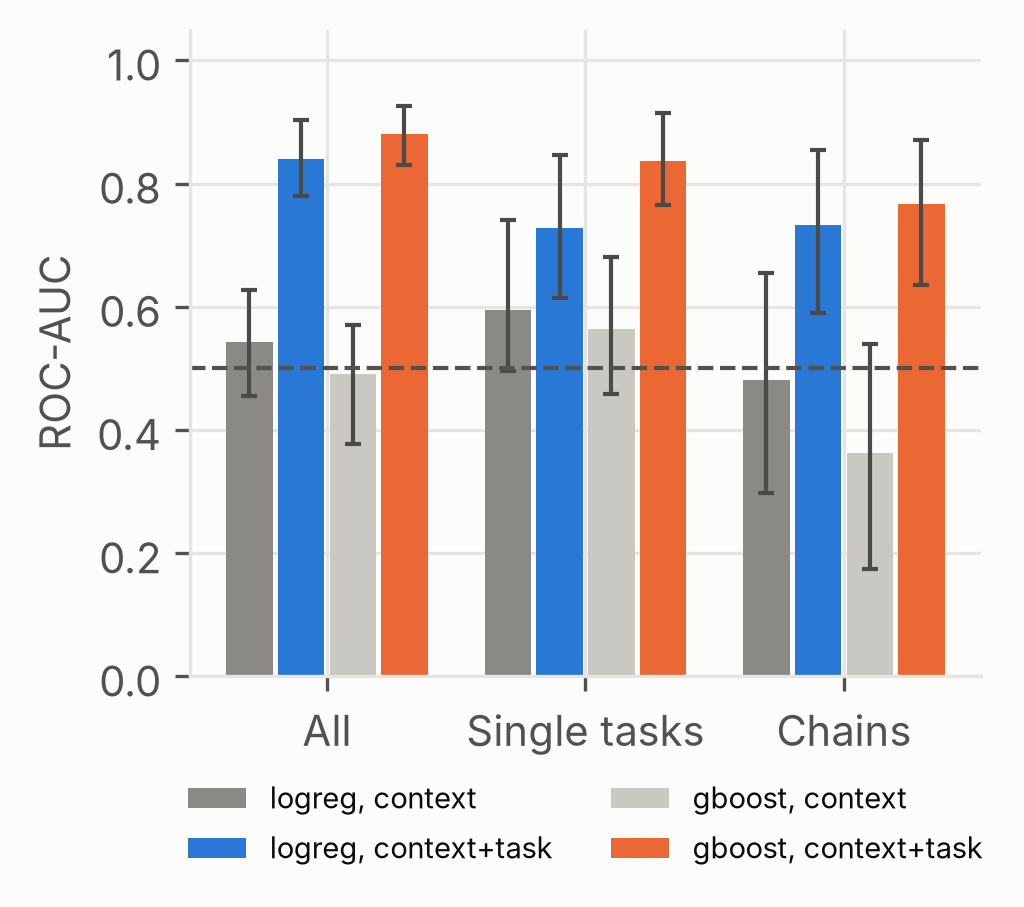
\includegraphics[width=0.85\columnwidth]{fig6_classifier.png}
\caption{Unreliable-task classifier, leave-one-task-out AUC with 95\% intervals. ``Context'' is the run setting;
``task'' adds the task descriptors. Dashed line: chance.}\label{fig:clf}
\end{figure}

\begin{figure}[t]
\centering
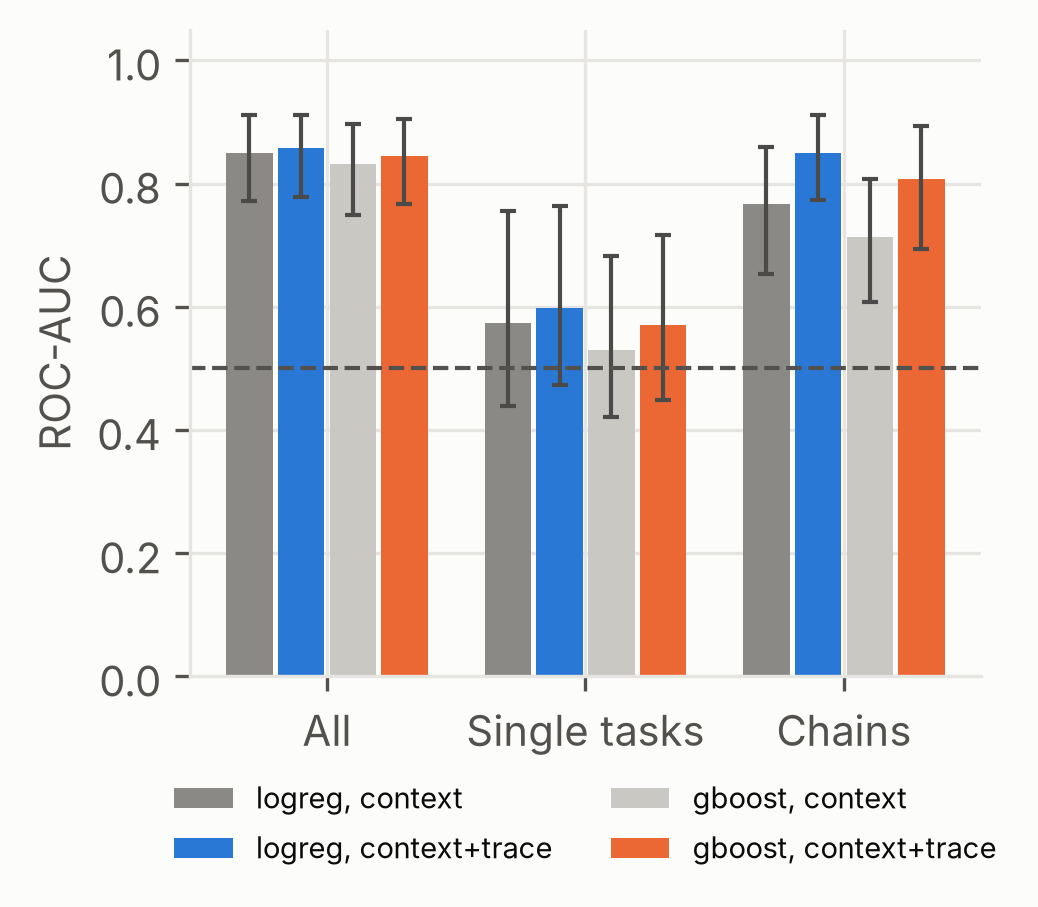
\includegraphics[width=0.85\columnwidth]{fig7_detector.png}
\caption{Failed-episode detector, leave-one-task-out AUC with 95\% intervals. ``Trace'' adds trace features to the run
setting. They help on chains and barely on single tasks.}\label{fig:det}
\end{figure}

\section{Discussion}
The first practical lesson is to report $\passk{k}$ next to pass@1, and to run enough trials for $k$ to be meaningful.
On clean single tasks the two differ by 0.03 to 0.05, so the extra column looks redundant. Under 20\% faults the gap
between pass@1 and $\passk{10}$ grows to 0.24 for 120b and 0.41 for 20b, and a deployment that must handle the same
request correctly every time experiences the $\passk{k}$ number. This agrees with what $\tau$-bench and the OSWorld study
report on very different tasks~\cite{taubench,cua}.

The second is that single-task suites do not predict multi-request behaviour. Both models looked strong on single tasks
and failed almost completely on four requests in one conversation. The failure is structural (stopping early and
over-claiming) rather than an accumulation of independent slips, so it should be tested directly. A cheap check that
compares the agent's claims with tool confirmations, together with a plan that forces a lookup before every decision,
recovered much of the loss on four-request chains, at about twice the tokens of a single task. It did not help on the
three-request chains we tested. Because these agents also misreport what they did, a score that checked the final reply
as well as the database would probably come out lower than ours.

Third, five runs per task is a minimum, not a comfortable budget. With ten runs, a ranking of settings agreed with the
full data on average from five runs, but some subsets of eight runs still reordered it, and close pairwise comparisons
never settled. Reports that compare agents from a single run per task can easily reach the wrong conclusion.

Finally, model size seemed to matter most under stress, though the evidence is still thin. At $\lambda=0.2$ the 20b
model reaches pass@1 0.81 against 0.94 for the 120b, and $\passk{10}$ 0.40 against 0.70, but with ten tasks the
$\passk{5}$ intervals overlap, so we read this as a direction and not a settled gap. The extra agent machinery mattered
more than model size on the longest chains: plan-then-execute with gpt-oss-20b (0.50) beat ReAct with gpt-oss-120b
(0.05). ReliabilityBench found that a simpler architecture held up better than Reflexion under stress~\cite{reliabilitybench};
in our data the added plan and audit helped on four-request chains and were neutral on single tasks, which suggests the
benefit of extra agent machinery depends on which failure it targets.

\section{Limitations}
The samples are small: four or eight chains per length, ten runs for the ReAct stress conditions, and five for E1 and
for plan-then-execute, whose comparison with ReAct rests on four chains per length. The plan-then-execute length-3 result
is reported from its run summary and is not in the other analyses. The planner was revised twice after reading traces
of the same chains it was then evaluated on, so its chain results may be optimistic for unseen chains. Injected faults
always fire before the tool runs, so retrying is safe. A timeout after the side effect has already happened is harder and
is not tested here. Paraphrase and fault experiments use one task set that both models solve perfectly when undisturbed,
which limits how much they can drop on pass@1. Chains were frozen before the third task set existed and use only the first
two. Success is judged on the final database, not on what the agent tells the customer, so a correct action with a
misleading reply still counts as a success. Token costs were logged only for the plan-then-execute reruns and the pilot.
The third model family is a six-episode pilot. Finally, all main results come from one environment and one model family
served by one provider.

\section{Conclusion}
In a small but fully checkable shop environment, a single success rate overstated how reliably two gpt-oss models handle
customer requests, especially under tool faults and when several requests share one conversation. Ten runs exposed
unreliability that five runs partly hid. Four-request chains failed far more often than independent errors predict,
because the agent tends to stop early and report work it never did. A plan that forces lookups, followed by an audit of
claimed actions against tool confirmations, raised four-request chain success from 0.05 to 0.70 (120b) and from 0.00 to
0.50 (20b), at a measurable token cost. Our next steps are to separate the planning and audit components with an
ablation, run plan-then-execute on more chains and seeds, test chains built from the third task set and a second model
family at full scale, and score the agent's final reply as well as the database.

\section*{Code and Data Availability}
All tasks, paraphrases, chains, episode logs, analysis scripts and figures are in the project repository.
\texttt{python check\_all.py} runs 16 offline checks, and \texttt{python replay\_sample.py --check} replays a small
cached sample of episodes without API calls. The analysis scripts regenerate every table and figure in this paper from
the logs, also without API calls.

\begin{thebibliography}{99}
\footnotesize
\setlength{\itemsep}{0pt}
\bibitem{swebench} C.~E. Jimenez, J.~Yang, A.~Wettig, S.~Yao, K.~Pei, O.~Press, and K.~Narasimhan, ``SWE-bench: Can
language models resolve real-world GitHub issues?,'' in \emph{Proc. Int. Conf. Learn. Represent. (ICLR)}, 2024.
\bibitem{taubench} S.~Yao, N.~Shinn, P.~Razavi, and K.~Narasimhan, ``$\tau$-bench: A benchmark for tool-agent-user
interaction in real-world domains,'' in \emph{Proc. Int. Conf. Learn. Represent. (ICLR)}, 2025.
\bibitem{metr} T.~Kwa \emph{et al.}, ``Measuring AI ability to complete long software tasks,'' in \emph{Advances in
Neural Information Processing Systems (NeurIPS)}, vol.~38, 2025.
\bibitem{kdd} M.~Mohammadi, Y.~Li, J.~Lo, and W.~Yip, ``Evaluation and benchmarking of LLM agents: A survey,'' in
\emph{Proc. 31st ACM SIGKDD Conf. Knowl. Discovery Data Mining (KDD)}, Toronto, ON, Canada, 2025, doi:
10.1145/3711896.3736570.
\bibitem{yehudai} A.~Yehudai \emph{et al.}, ``Survey on evaluation of LLM-based agents,'' arXiv:2503.16416, 2025.
\bibitem{reliabilitybench} A.~Gupta, ``ReliabilityBench: Evaluating LLM agent reliability under production-like stress
conditions,'' arXiv:2601.06112, 2026.
\bibitem{cua} G.~Gonzalez-Pumariega, S.~Agashe, J.~Yang, A.~Li, and X.~E. Wang, ``On the reliability of computer use
agents,'' arXiv:2604.17849, 2026.
\bibitem{gabauer} C.~Gabauer, ``LLM-based agent systems: A systematic literature review and position on hybrid
architectures and evaluation frameworks,'' \emph{Appl. Intell.}, vol.~56, no.~10, Art. no.~325, 2026, doi:
10.1007/s10489-026-07340-9.
\bibitem{chowa} S.~S. Chowa \emph{et al.}, ``From language to action: A review of large language models as autonomous
agents and tool users,'' \emph{Artif. Intell. Rev.}, vol.~59, no.~2, Art. no.~71, 2026, doi: 10.1007/s10462-025-11471-9.
\bibitem{androidarena} M.~Xing, R.~Zhang, H.~Xue, Q.~Chen, F.~Yang, and Z.~Xiao, ``Understanding the weakness of large
language model agents within a complex Android environment,'' in \emph{Proc. 30th ACM SIGKDD Conf. Knowl. Discovery Data
Mining (KDD)}, 2024, pp.~6061--6072.
\bibitem{react} S.~Yao, J.~Zhao, D.~Yu, N.~Du, I.~Shafran, K.~Narasimhan, and Y.~Cao, ``ReAct: Synergizing reasoning and
acting in language models,'' in \emph{Proc. Int. Conf. Learn. Represent. (ICLR)}, 2023.
\bibitem{reflexion} N.~Shinn \emph{et al.}, ``Reflexion: Language agents with verbal reinforcement learning,'' in
\emph{Advances in Neural Information Processing Systems (NeurIPS)}, vol.~36, 2023.
\bibitem{planandsolve} L.~Wang \emph{et al.}, ``Plan-and-solve prompting: Improving zero-shot chain-of-thought reasoning
by large language models,'' in \emph{Proc. 61st Annu. Meeting Assoc. Comput. Linguistics (ACL)}, 2023.
\bibitem{codex} M.~Chen \emph{et al.}, ``Evaluating large language models trained on code,'' arXiv:2107.03374, 2021.
\bibitem{gptoss} OpenAI, ``gpt-oss-120b \& gpt-oss-20b model card,'' arXiv:2508.10925, 2025.
\bibitem{wilson} E.~B. Wilson, ``Probable inference, the law of succession, and statistical inference,'' \emph{J. Amer.
Statist. Assoc.}, vol.~22, no.~158, pp.~209--212, 1927.
\bibitem{kendall} M.~G. Kendall, ``A new measure of rank correlation,'' \emph{Biometrika}, vol.~30, no.~1/2,
pp.~81--93, 1938.
\bibitem{sklearn} F.~Pedregosa \emph{et al.}, ``Scikit-learn: Machine learning in Python,'' \emph{J. Mach. Learn.
Res.}, vol.~12, pp.~2825--2830, 2011.
\end{thebibliography}

\end{document}
